\documentclass[a4paper,12pt]{scrartcl}
\usepackage[utf8]{inputenc}
\usepackage{amsmath}

\usepackage{graphicx}
\usepackage{caption}
\usepackage{subcaption}
\usepackage[left=3cm,right=3cm,top=3.5cm,bottom=3.5cm]{geometry}
\usepackage{pgfplots,pgfplotstable}
\usepackage{tikz}
%\usetikzlibrary{positioning, fadings, through}
\usepackage{fancyhdr}
\usepackage[locale=DE,output-decimal-marker={.}]{siunitx}
\sisetup{separate-uncertainty, per-mode=fraction,}
\usepackage{here}
\usepackage{hyperref}

\usepackage{setspace}
\onehalfspacing
\usepackage{comment}

\usepackage{circledsteps}

% Default fixed font does not support bold face
\DeclareFixedFont{\ttb}{T1}{txtt}{bx}{n}{12} % for bold
\DeclareFixedFont{\ttm}{T1}{txtt}{m}{n}{12}  % for normal

% Custom colors
\usepackage{color}
\definecolor{deepblue}{rgb}{0,0,0.5}
\definecolor{deepred}{rgb}{0.6,0,0}
\definecolor{deepgreen}{rgb}{0,0.5,0}

\usepackage{listings}

% Python style for highlighting
\newcommand\pythonstyle{\lstset{
numbers=left,
language=Python,
basicstyle=\ttm,
otherkeywords={self},             % Add keywords here
keywordstyle=\ttb\color{deepblue},
emph={MyClass,__init__},          % Custom highlighting
emphstyle=\ttb\color{deepred},    % Custom highlighting style
stringstyle=\color{deepgreen},
frame=tb,                         % Any extra options here
showstringspaces=false            % 
}}


% Python environment
\lstnewenvironment{python}[1][]{
\pythonstyle
\lstset{#1}
}{}

% Python for external files
\newcommand\pythonexternal[2][]{{
\pythonstyle
\lstinputlisting[#1]{#2}}}

% Python for inline
\newcommand\pythoninline[1]{{\pythonstyle\lstinline!#1!}}


\usepackage{booktabs}
\usepackage{multirow}
\usetikzlibrary{external}
\tikzexternalize[prefix=tikz/]

\pgfplotsset{compat=newest,
    tick label style={font=\small},
    label style={font=\small},
    legend style={font=\footnotesize}
    }
    
\tikzset{every mark/.append style={scale=0.3}}
\tikzset{>=stealth}
\usepackage{acronym}
\newlength{\plotheight}
\newlength{\plotwidth}
\newlength{\imgheight}
\setlength{\plotwidth}{14cm}
\setlength{\plotheight}{8cm}


\newcommand{\titel}{Finite Difference Mode Solver}
\usepackage{fancyhdr}
\fancyhf{}
\pagestyle{fancy}
\cfoot{\thepage}
\fancyhead[L]{\leftmark}
\fancyhead[R]{\thepage}

\subject{Report}
\title{\titel}
\author{\Large{Steev \textsc{Mathew}, Felix \textsc{Wechsler}, Yaqi \textsc{Zhang}}\\  \large{Group 3}}
\date{\large{\today}}
\publishers{\vspace{5.5cm}Abbe School of Photonics\\
            Friedrich-Schiller-Universität Jena}


\newcommand\todo[1]{\textcolor{red}{\textbf{TODO: #1}}}

%proper Integral typsetting
\newcommand{\dt}{\, \mathrm{d}t}
\newcommand{\dd}{\mathrm{d}}

\newcommand\ff[1]{ \mathbf #1(\mathbf r, \omega)}
\newcommand\lap{\mathop{{}\bigtriangleup}\nolimits}

\usepackage[%
  backend=biber,
  url=false,
  style=alphabetic,
  % citestyle=authoryear,
  maxnames=4,
  minnames=3,
  maxbibnames=99,
  giveninits,
uniquename=init]{biblatex}

\addbibresource{references.bib}
\pgfkeys{/csteps/inner color=transparent , /csteps/outer color=black}


%indentation to 0
\setlength\parindent{0pt}
\begin{document}
    \maketitle
	\thispagestyle{empty}
	\newpage
	\tableofcontents

\newpage
\section{Introduction}
    In this report we explain how we can create a simple finite difference mode
    solver in \texttt{Python}.
    The physical problem we solve as an example, is the calculation
    of guided modes in 2D and 3D media. 
    For simplification we assume low gradients in the dielectric permittivity and hence we solve the stationary scalar Helmholtz equation.

\section{Physical Background}
    In this section we introduce the main physical concept. A more extensive discussion can be found in \cite{lecture}.
    Starting from Maxwell's equation, we can derive the general wave equation:
    \begin{align}
        \nabla \times \nabla \times \mathbf E(\mathbf r, \omega) = \frac{\omega^2}{c^2} \varepsilon(\mathbf r, \omega) \mathbf E(\mathbf r, \omega)
        \label{eq:wave}
    \end{align}
    Assuming that the change in $\varepsilon$ is rather small, we can write:
    \begin{align}
        \nabla \cdot \ff D = 0 \Rightarrow \varepsilon(\mathbf r, \omega) \nabla \cdot \ff E \approx 0
    \end{align}
    This simplifies the wave equation to the Helmholtz equation:
    \begin{align}
        \lap \ff E + \frac{\omega^2}{c^2} \varepsilon(\mathbf r, \omega) \ff E = 0
        \label{eq:helm}
    \end{align}
    The general 3D ansatz functions for a wave propagation in $z$-direction for the Helmholtz equation are plane waves in the form of:
    \begin{align}
        \ff E = \mathbf E_0(x, y) \exp\left[i \beta(\omega) z - i \omega t\right]
        \label{eq:ansatz}
    \end{align}
    Inserting \autoref{eq:ansatz} into \autoref{eq:helm} provides the final result we need for the numerical calculation of the eigenmodes:
    \begin{align}
        \frac1{k_0^2} \left(\frac{\partial^2}{\partial x^2}+ \frac{\partial^2}{\partial y^2}\right) E_0(x,y, \omega)+ \varepsilon(x, y, \omega) E_0(x, y, \omega) = \varepsilon_{\text{eff}}(\omega) E_0(x, \omega)
        \label{eq:final}
    \end{align}
    where $\varepsilon_{\text{eff}}=\left(\frac{\beta(\omega)}{k_0}\right)^2$
    and $k_0 = \frac{2\pi}{\lambda}$ and $\lambda$ being the wavelength of the electric field.
    On the left hand side of \autoref{eq:final} we see a second spatial derivative regarding $x$ and $y$.
    The time dependency can be left out, since we are looking for stationary modes and the time dependency is just trivial.
    
\section{Numerical Implementation}
    First we show the numerical background and afterwards we explain some details of our implementation.
    \subsection{Background}
    We directly explain the numerical discretization in 2D since 1D is only a special case of it. For simplicity we split the continuous space into a 2D grid with size $N_y \times N_x$. In \autoref{fig:disc} we see such a discretization.
     \begin{figure}[h]
        \centering
        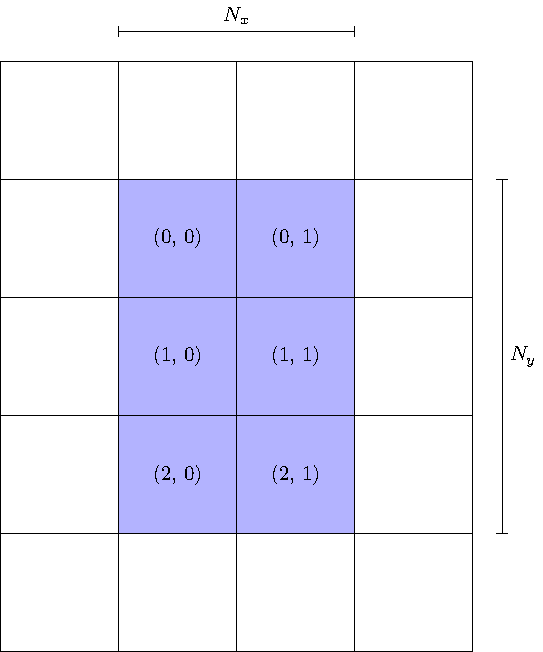
\includegraphics[width=.5\textwidth]{figures/2d-grid.pdf}
        \caption{Discretization of the space}
        \label{fig:disc}
    \end{figure}
    
    The function $f(x, y)$ is now represented by samples $f_{i,j}$.
    The central finite difference to calculate the second derivative is given by the following equation:
    \begin{align}
        \frac{\partial^2 f}{\partial x^2}  + \frac{\partial^2 f}{\partial y^2} \bigg|_{x_i, y_j} \approx 
        \frac{f_{i+1, j} + f_{i-1, j} + f_{i, j+1} + f_{i, j-1} - 4 f_{i, j}}{h^2}
        \label{eq:disc}
    \end{align}
    We assume that the boundary of the function $f$ is zero. The white cells are 0 and the blue cells are non restricted. This simplifies the second derivative for blue cells which have
    neighbouring white cells.
    Following \autoref{eq:disc} we can express this equation via a matrix vector multiplication:
    \begin{align}
        \frac{\partial^2 f}{\partial x^2}  + \frac{\partial^2 f}{\partial y^2}  \approx \frac{1}{h^2}
        \begin{bmatrix}
            -4 & 1  & 1  &    &    & \\ 
             1 & -4 & 0  & 1  &    &  \\
             1 & 0  & -4 & 1  & 1  & \\
               & 1  & 1  & -4 & 0  & 1 \\
               &    & 1  & 0  & -4 & 1 \\
               &    &    & 1  & 1  & -4 
        \end{bmatrix} \cdot       
        \begin{bmatrix}
            f_{0,0} \\ f_{0,1} \\ f_{1,0} \\ f_{1,1 } \\ f_{2,0} \\ f_{2,1} 
        \end{bmatrix}
    \end{align}
    $h$ must be set to the discretization sampling.
    This scheme can be extended to a higher number of grid points. 
    There are certain rules this matrix obeys. The diagonal elements are always of -4.
    The off diagonals $x_{m+1, m}$ with $m \in \{0, 1, \dots, N_x + N_y - 2\}$ 
    and $x_{n, n+1}$ with $n \in \{0, 1, \dots, N_x + N_y - 2\}$ are always 1 expect when
    $(m+1) \equiv 0 \,  \mathrm{mod} \, N_x$ and  $(n+1) \equiv 0 \, \mathrm{mod} \, N_x$. This handles
    the case of the line break of the 2D grid. The vector consists of the $x$-rows of the grid. 
    They have an offset of $N_x$ to the main diagonal. This is again due to the line break. 
    The elements are always 1.
    Having expressed the Laplacian as a matrix we can write down \autoref{eq:final} in this form:
    \begin{align*}
    &                 \scriptstyle 
        \begin{bmatrix}
            - \frac{4}{k_0^2 h^2} + \varepsilon_{0,0} & \frac{1}{k_0^2 h^2}  & \frac{1}{k_0^2 h^2}  &    &    & \\ 
             \frac{1}{k_0^2 h^2}& - \frac{4}{k_0^2 h^2} + \varepsilon_{0,1} & 0  & \frac{1}{k_0^2 h^2}  &    &  \\
             \frac{1}{k_0^2 h^2} & 0  & - \frac{4}{k_0^2 h^2} + \varepsilon_{1,0} & \frac{1}{k_0^2 h^2}  & \frac{1}{k_0^2 h^2}  & \\
               & \frac{1}{k_0^2 h^2}  & \frac{1}{k_0^2 h^2}  & - \frac{4}{k_0^2 h^2} + \varepsilon_{1,1} & 0  & \frac{1}{k_0^2 h^2} \\
               &    & \frac{1}{k_0^2 h^2} & 0  & - \frac{4}{k_0^2 h^2} + \varepsilon_{2,1} & \frac{1}{k_0^2 h^2} \\
               &    &    & \frac{1}{k_0^2 h^2}  & \frac{1}{k_0^2 h^2}  & - \frac{4}{k_0^2 h^2} + \varepsilon_{2,2} 
        \end{bmatrix} \cdot \\ &\begin{bmatrix}
            E_{0,0} \\ E_{0,1} \\ E_{1,0} \\ E_{1,1 } \\ E_{2,0} \\ E_{2,1} 
        \end{bmatrix}  = \varepsilon_{\text{eff}}\begin{bmatrix} E_{0,0} \\ E_{0,1} \\ E_{1,0} \\ E_{1,1 } \\ E_{2,0} \\ E_{2,1} \end{bmatrix}
        \label{eq:final}
    \end{align*}
    To solve for the vector $E_{i,j}$ we need to solve an eigenvalue problem. 
    
    \subsection{Implementation}
    In this part we explain important steps of our source code. The full code can be found in the attachment.
    Important to note is, that we use the function \pythoninline{diags} from the \pythoninline{scipy.sparse} package \cite{2020SciPy-NMeth}. This allows us to create a sparse matrix with the diagonals stored in \pythoninline{data} and with offsets \pythoninline{[0, 1, -,1 -Nx, Nx]}. A dense matrix would not be possible to store
    for 3D problems.
    One important step is the creation of a mask in line 135. This is needed, as we have seen before
    that the off diagonals have zeros at certain positions. This is achieved by that mask.
    In line 137 we set the off diagonals to 0 where the mask is true.
    
    Having that matrix finally created with line 144, we can call the function\\
    \pythoninline{get_eigen_matrix}.
    This function essentially calls \pythoninline{eigsh} from \pythoninline{scipy.sparse} to calculate 
    the eigenvectors and eigenvalues of our matrix. 
    Furthermore we take the real part of both the eigenvectors and eigenvalues.
    This is reasonable assuming that our material is lossless. Another issue arising from \pythoninline{eigsh} is, that the eigenvalues are not ordered. Therefore we perform an additional
    sorting of the eigenvectors and eigenvalues.
    The reason why we use \pythoninline{eigsh} instead of \pythoninline{eigs} is speed.
    The latter turns out to be slower on our type of problem. Since the matrix is symmetric, we can use
    the symmetric version \pythoninline{eigsh}.
    
\newpage
\section{Results}
    In this section we present the obtained results.
    In \autoref{fig:1D} we can see the numerical results for the 2D slab material. 
    We only show five solutions with the highest effective $\varepsilon_\text{eff}$. It can be seen that the ground mode is associated with the highest effective permittivity.
    The normalization is chosen in such a way, that the peaks are 1. 
    \begin{figure}[H]
        \centering
        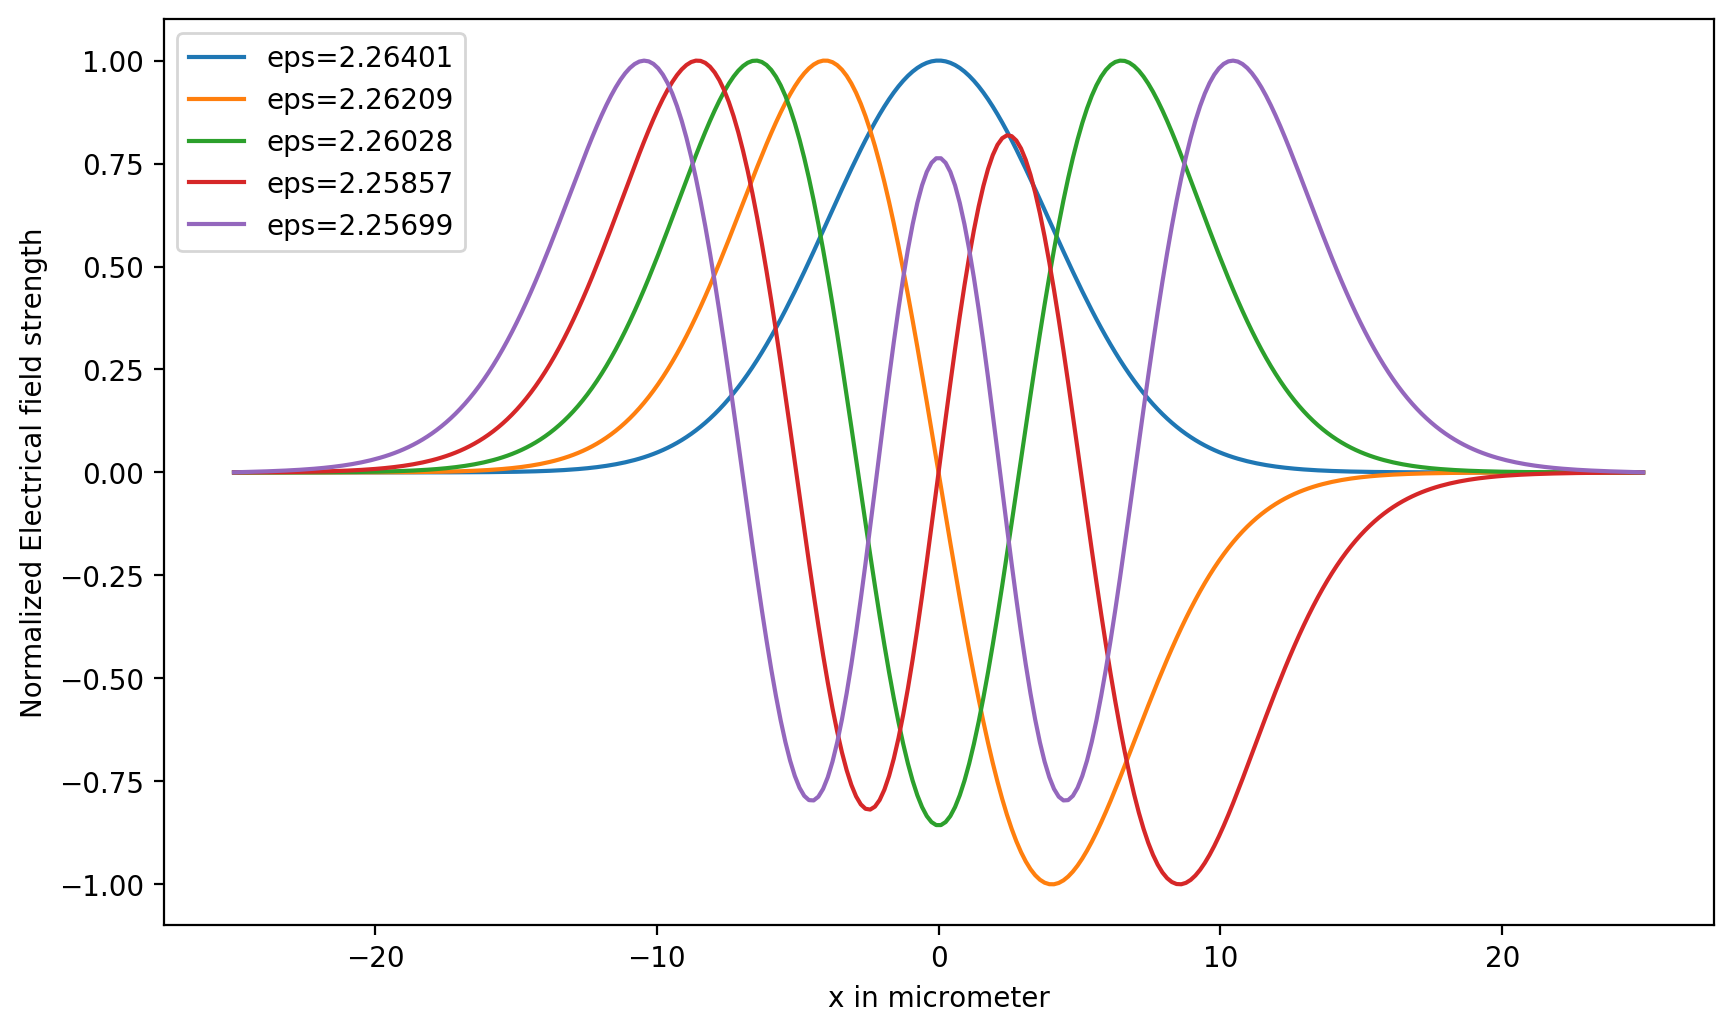
\includegraphics[width=.9\textwidth]{figures/1D.png}
        \caption{The first 5 modes in a slab waveguide.}
        \label{fig:1D}
    \end{figure}
    Important for a correct numerical solution is, that the grid is large enough that the modes are already close to 0 at the boundary. A grid of $[\SI{-10}{\micro\meter}, \SI{10}{\micro\meter}]$ for example would not be broad enough to ensure that the field is 0. Additionally, as it can be seen, higher order modes are spatially more extended.
    
    In \autoref{fig:2D} and \autoref{fig:2Dh} we can see the 2D cross section of the normalized
    electrical field for the 3D waveguide.
    The 0th order is symmetric around the center. The 2nd order is not.  
    \begin{figure}[H]
        \centering
        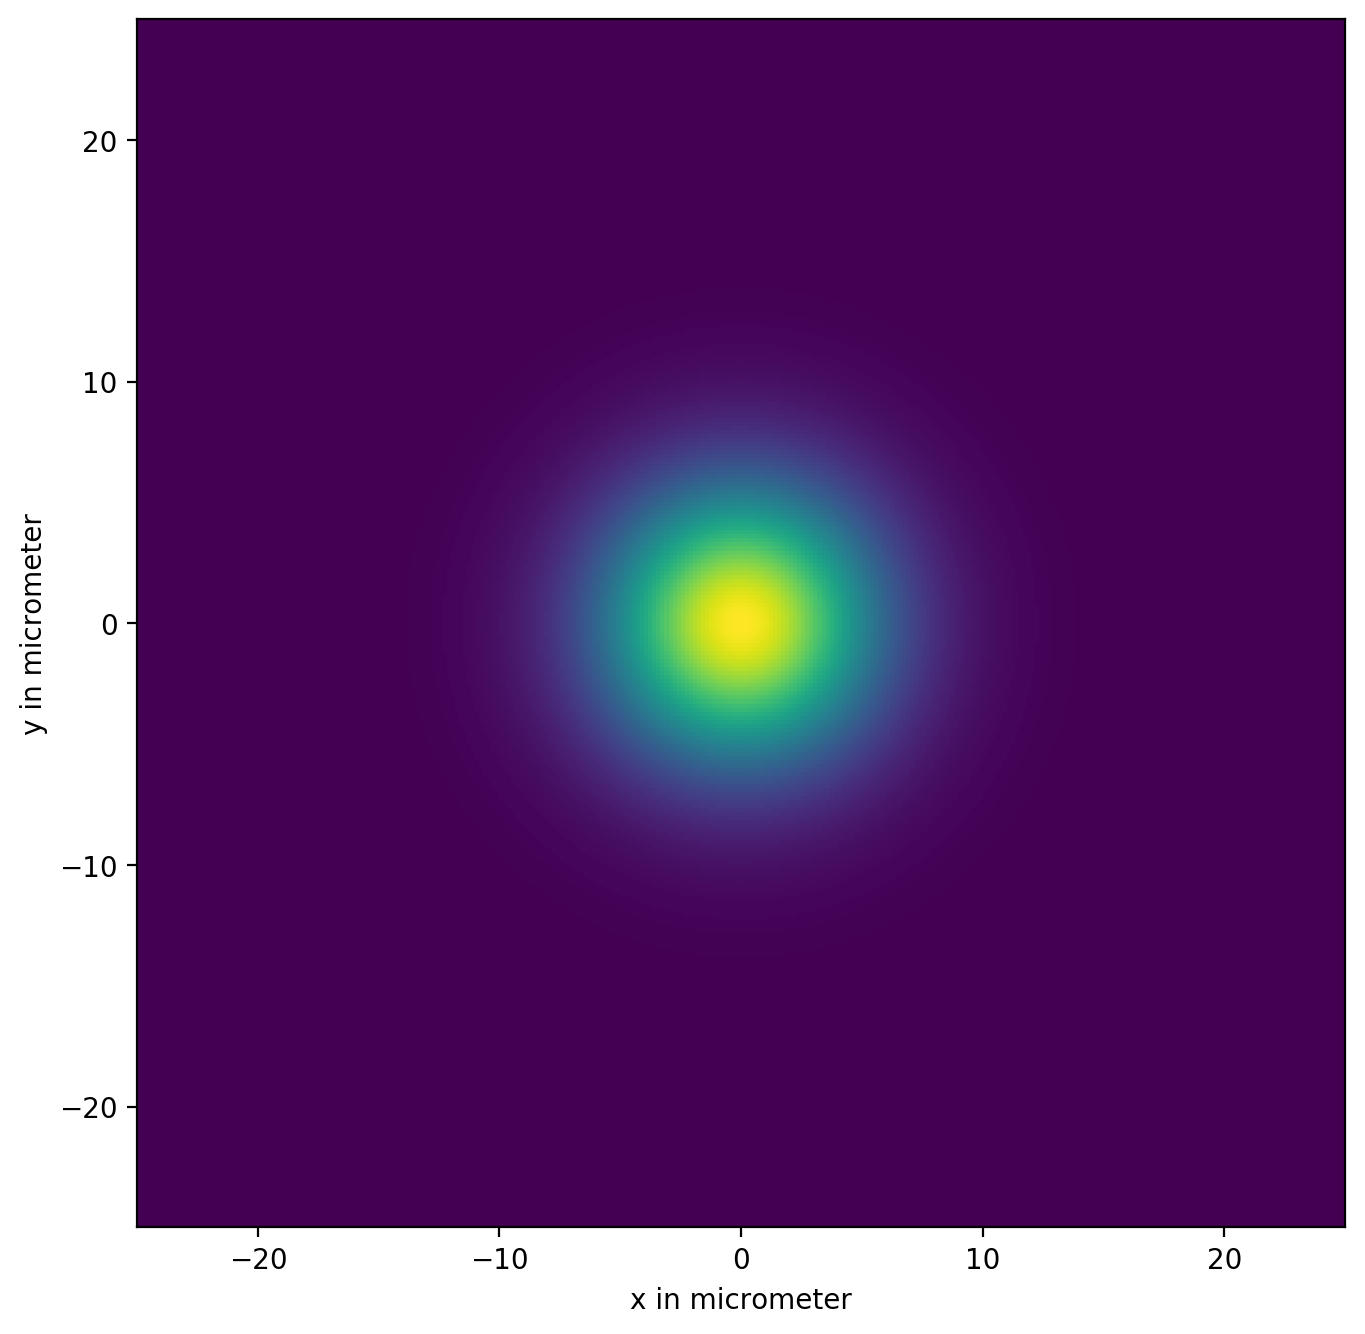
\includegraphics[width=.6\textwidth]{figures/2D.png}
        \caption{The first mode (0th order) in a strip waveguide.}
        \label{fig:2D}
    \end{figure}
    We notice that this 2nd order mode is also rotated slightly and is not aligned with the symmetry of the grid. This is reasonable since the modes are not oriented in a specific way. Also \pythoninline{eigsh} returns different orientations if it is called multiple times.
    
       \begin{figure}[H]
        \centering
        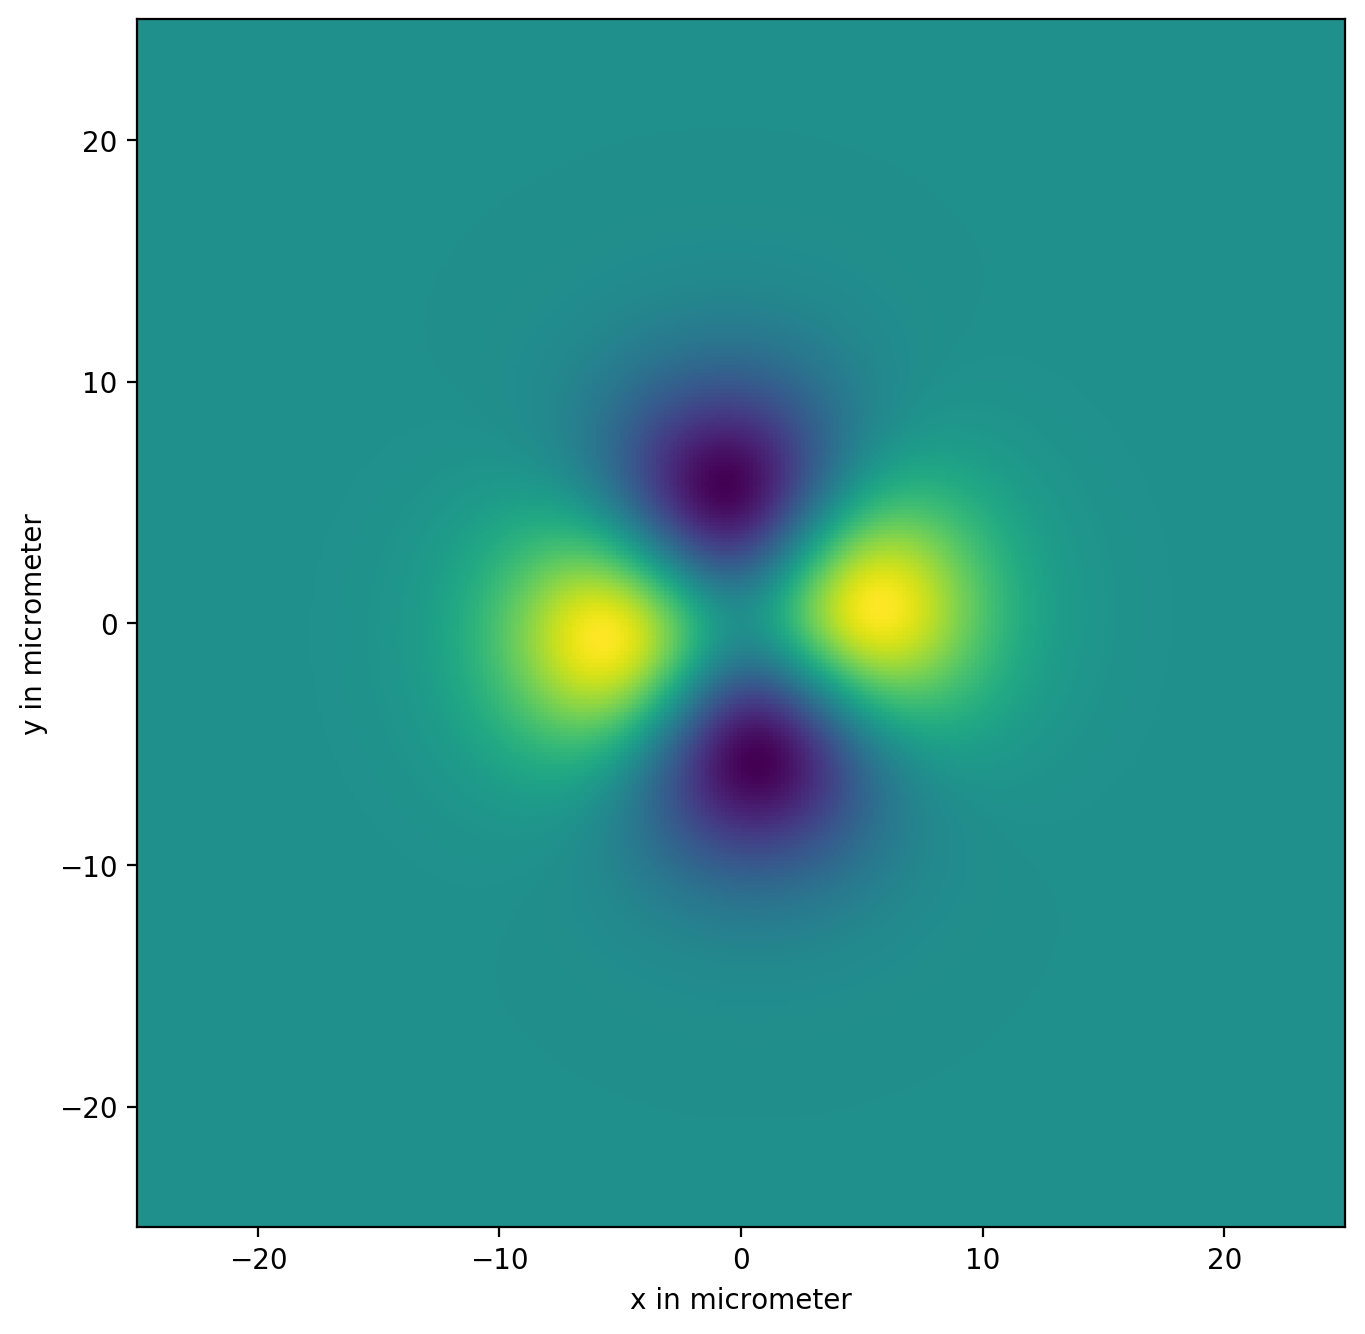
\includegraphics[width=.6\textwidth]{figures/2D_higher.png}
        \caption{A higher order mode (2nd order) in a strip waveguide.}
        \label{fig:2Dh}
    \end{figure}
    
    Our source code is also designed in a way to calculate non-rectangular grids.
    This is useful if one wants to solve systems which require more data points 
    in a certain direction. An example is shown in \autoref{fig:2Dnr}.
         \begin{figure}[H]
        \centering
        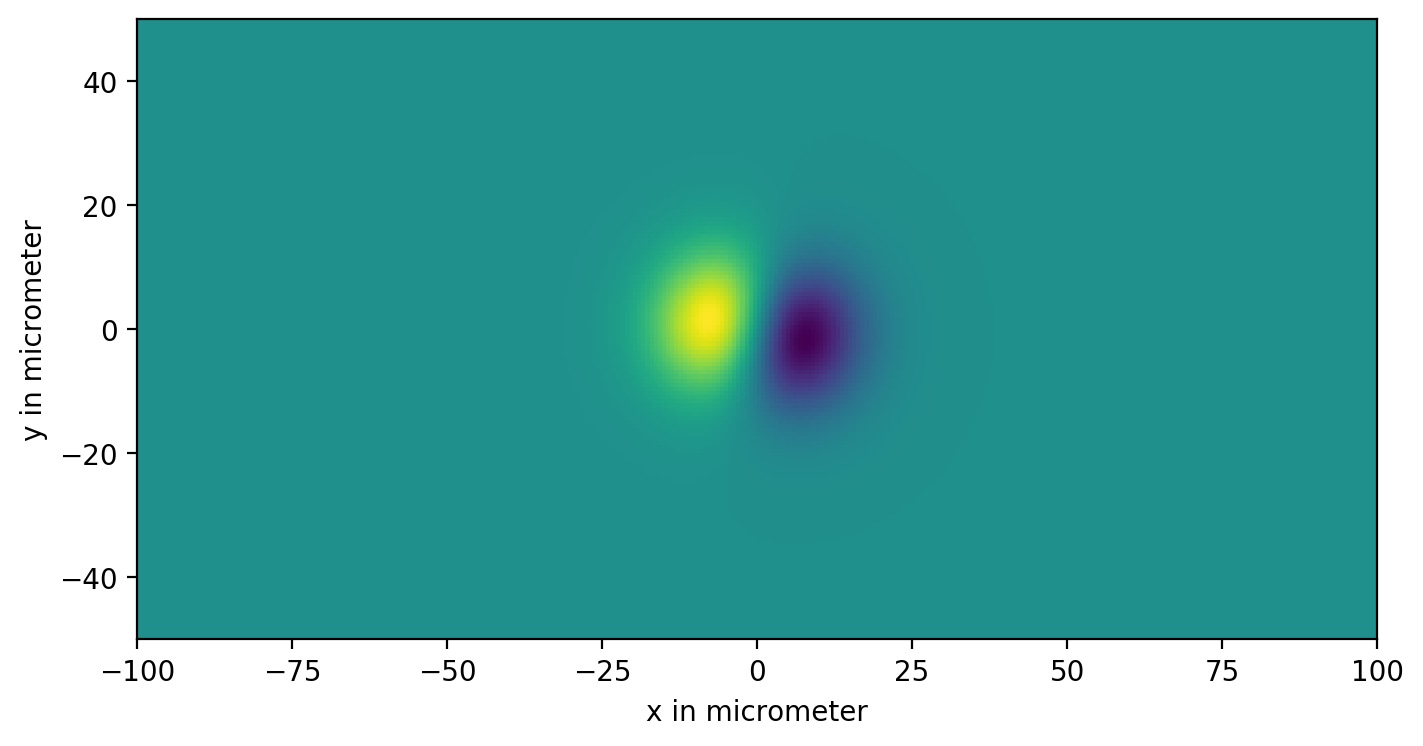
\includegraphics[width=.6\textwidth]{figures/2D-nonrect.png}
        \caption{A higher order mode (1st order) in a strip waveguide on a non-rectangular grid.}
        \label{fig:2Dnr}
    \end{figure}
    
    \subsection{Speed}
        We also measured the time needed to calculate the eigenmodes. 
        Our setup for all measurements was Python 3.8.2, SciPy 1.3.2, NumPy 1.17.3 and a Intel(R) Core(TM) i7-7600U CPU @ 2.80GHz.
        The full results can be found in \autoref{tab:res}.
        Whether using single or double precision did make a significant difference in the slab waveguide.
        Unexpected was, that single precision was actually slower.
        \begin{table}[h]
            \setstretch{1.5}
            \begin{tabular}{l r r}
               & Time needed for \pythoninline{eigsh} in \si{\second}  & Total time needed in \si{\second}  \\
               \hline
                2D, single precision &  $0.2\pm 0.04$ & $0.21 \pm 0.04$ \\
                2D, double precision &  $0.13\pm 0.02$ & $0.14 \pm 0.02$ \\
                \hline
                3D, single precision &  $2.64\pm 0.16$ & $2.65 \pm 0.16$ \\
                3D, double precision &  $13.43\pm 0.98$ & $13.44 \pm 0.97$ \\
            \end{tabular}
            \caption{Results for the computing time}
            \label{tab:res}
        \end{table}
        For a 3D material, the time difference between single and double precision was significant.
        In both cases the numerical results were up to machine precision identical. 
        The exact chosen parameters for both runs can be found in the attached Jupyter Notebook.
        Another characteristic of the algorithm is, that it takes more time to compute more eigenmodes. To calculate the first mode, it is therefore usually enough to calculate
        one eigenvalue. This reduces the computational time further.
        In \autoref{tab:res} we list also the time needed in the function \pythoninline{eigsh}. This function call needs most of the computational time, which is also expected since it does all the solving part. This indicates that our source code performs well and is not the bottleneck.

        
\section{Conclusion}
In this report we presented a quick introduction into finite difference mode solver. Attached to this report the full source code can be found.
Using the code, we were able to reproduce different guided modes. We have to show that single precision results are beneficial to use in the 3D case and give a significant speedup without loss of physical relevant accuracy.


%\section{Attachment}
%    \pythonexternal{code/full.py}
    
\newpage
%to print all entries
\nocite{*}
\printbibliography


\end{document}